%%%%%%%%%%%%%%%%%%%%%%%%%%%%%%%%%%%%%%%%%%%%%%%%%%%%%%%%%%%%
\documentclass[11pt,            % Schriftgröße {{{
               a4paper,         % A4
               oneside,         % Einseitig
               DIV12,           % Papiergröße
             % DIV15,           % Größer
             % draft,           % Entwurf
               fleqn,           % Linksbündige Gleichungen
             % headsepline,     % Trennlinie oben
             % footsepline,     % -""-       unten
             % smallheadings,   % Kleine Überschriften
             % pointlessnumbers,% Keine Punkte
               halfparskip,     % Halbe Zeile Absatz statt Einzug
               nochapterprefix, % Kein "Kapitel"
             % bibtotoc         % "Literatur" im TOC  oder
             % bibtotocnumbered,% -""-, nummeriert
             % idxtotoc,        % Index im TOC
              ]{scrartcl} %%% }}}
%%%%%%%%%%%%%%%%%%%%%%%%%%%%%%%%%%%%%%%%%%%%%%%%%%%%%%%%%%%%

%%%%%%%%%%%%%%%%%%%%%%%%%%%%%%%%%%%%%%%%%%%%%%%%%%%%%%%%%%%%
%%% Pakete {{{
\usepackage[utf8x]{inputenc}
\usepackage[greek,english]{babel}
\usepackage[T1]{fontenc}            % T1-kodierte Fonts
\usepackage{setspace}               % Single- oder Onehalfspacing
\setcounter{tocdepth}{4}            % 4 Hirarchien im Inhaltsv.
\usepackage{times}                  % Times als Schrift
\usepackage{amsmath,amssymb,amstext}% Mathematische Symbole
\usepackage{exscale}                % Skalierung von Summen-c und Int.-zeichen
\usepackage{url}                    % Darstellung von URLs
\usepackage{calc}

%%% Optional, je nach Dokument
% \usepackage{listings}             % Quelltext-Listings
% \usepackage{units}                % Technische Units
% \usepackage{psfrag}               % Ersetzts PS-Schriften
  \usepackage{color}                % Farben in LaTeX
% \usepackage{floatflt}             % Textumflossene Bilder...
% \usepackage{picins}               % Textumflossene Bilder
  \usepackage{textcomp}             % Spezielle Zeichen
  \usepackage{gensymb}              % Spezielle Zeichen
% \usepackage{eurosym}              % Euro-Symbol
% \usepackage{currvita}             % Befehle für CVs
  \usepackage{ifpdf}                % Wird ein PDF erstellt?

% https://tex.stackexchange.com/questions/37581/latex-figures-side-by-side
  \usepackage{caption}
  \usepackage{subcaption}

  \usepackage{pdflscape}

%%% Layout
\usepackage{scrpage2}               % KOMA-Überschriften und -Fußzeilen.
%%% }}}
%%%%%%%%%%%%%%%%%%%%%%%%%%%%%%%%%%%%%%%%%%%%%%%%%%%%%%%%%%%%

%%%%%%%%%%%%%%%%%%%%%%%%%%%%%%%%%%%%%%%%%%%%%%%%%%%%%%%%%%%%
%%% PDF {{{

\ifpdf
  \usepackage[pdftex]{graphicx}
  \usepackage{float}
  \DeclareGraphicsExtensions{.pdf}
  \pdfcompresslevel=9
  \usepackage[%
    pdftex=true,
    backref=true,
    colorlinks=true,
    bookmarks=true,
    breaklinks=true,
    linktocpage=true,
    bookmarksopen=false,
    bookmarksnumbered=false,
    pdfpagemode=None
  ]{hyperref}
  \hypersetup{
    pdftitle={},
    pdfauthor={Julius Plenz},
    pdfsubject={},
    pdfcreator={LaTeX2e and pdfLaTeX},
    pdfproducer={},
    pdfkeywords={}
  }
\else
  \usepackage[dvips]{graphicx}
  \DeclareGraphicsExtensions{.eps}
  % \usepackage[%
  %   dvips,
  %   breaklinks=true,
  %   colorlinks=false
  % ]{hyperref}
\fi

%%% }}}
%%%%%%%%%%%%%%%%%%%%%%%%%%%%%%%%%%%%%%%%%%%%%%%%%%%%%%%%%%%%

%%%%%%%%%%%%%%%%%%%%%%%%%%%%%%%%%%%%%%%%%%%%%%%%%%%%%%%%%%%%
%%% Eigene Funktionen {{{
%%% Beispiel:  \bild{200pt}{foo}{That's a foo\ldots}
\newcommand{\bild}[3]{
  \begin{figure}
    \includegraphics[width=#1, keepaspectratio=true]{#2}
    \caption{#3}
    \label{#2}
  \end{figure}
}

%% \floatimg{filename}{caption+label}{r/l}{8cm}
\newcommand{\floatimg}[4]{
  \piccaption{#2}
  \parpic[#3]{\includegraphics[width=#4]{#1}}
}
%%% }}}
%%%%%%%%%%%%%%%%%%%%%%%%%%%%%%%%%%%%%%%%%%%%%%%%%%%%%%%%%%%%

%%%%%%%%%%%%%%%%%%%%%%%%%%%%%%%%%%%%%%%%%%%%%%%%%%%%%%%%%%%%
%%% Pagestyle {{{
  \pagestyle{scrheadings}
% \pagestyle{fancyhdrs}
% \pagestyle{empty}
%%% }}}
%%%%%%%%%%%%%%%%%%%%%%%%%%%%%%%%%%%%%%%%%%%%%%%%%%%%%%%%%%%%

%%%%%%%%%%%%%%%%%%%%%%%%%%%%%%%%%%%%%%%%%%%%%%%%%%%%%%%%%%%%
%%% Seitenkopf- und -Fußzeilen {{{
 \automark[subsection]{section} % \left- und \rightmark bekommen Inhalt
%%% Oben: Links, Mitte, Rechts
 \ihead[]{\rightmark}
 \chead[]{}
 \ohead[]{\pagemark}
%%% Unten: Links, Mitte, Rechts
 \ifoot[]{}
 \cfoot[]{}
 \ofoot[]{}
%%% }}}
%%%%%%%%%%%%%%%%%%%%%%%%%%%%%%%%%%%%%%%%%%%%%%%%%%%%%%%%%%%%

%%%%%%%%%%%%%%%%%%%%%%%%%%%%%%%%%%%%%%%%%%%%%%%%%%%%%%%%%%%%
%%% Sonstiges {{{
% \setlength{\parindent}{17pt}      % Einzug 17pt,
% \setlength{\parskip}{2pt}         % keine Leerzeilen.

% \textwidth      127mm             % Textbreite
% \textheight     235mm             % Texthöhe
% \topmargin     -5mm               % Abstand oben
% \oddsidemargin  7mm               % Abstand Links, onepage

%\onehalfspacing                    % Zeilenabstand: Bei korrektur,
 \singlespacing                     % bei Abgabe

% Punkt- und Komma Abstände bei Tausendern/
% Dezimalzahlen ans deutsche anpassen!
 \mathcode`,="013B
 \mathcode`.="613A

 \setlength{\emergencystretch}{2em} % Notfallsstreckung
 \addtolength{\voffset}{10pt}

% Kommandoänderungen
%\renewcommand{\figurename}{Abb.} % Bildunterschriften: Abb. anstatt Fig.
%\renewcommand*{\cvheadingfont}{\raggedleft\Huge\bfseries} % CV: Überschriften
%%% }}}
%%%%%%%%%%%%%%%%%%%%%%%%%%%%%%%%%%%%%%%%%%%%%%%%%%%%%%%%%%%%


\usepackage{amsthm}

\theoremstyle{definition}
\newtheorem*{beweis}{Beweis}
\newtheorem{definition}{Definition}
\newtheorem*{bemerkung}{Bemerkung}
\newtheorem*{beispiel}{Beispiel}


\begin{document}

%%%%%%%%%%%%%%%%%%%%%%%%%%%%%%%%%%%%%%%%%%%%%%%%%%%%%%%%%%%%
%%% Titelseite {{{
\pagenumbering{none}                % Für die Titelseite: Keine Seitennummern,
\thispagestyle{empty}               % keine Kopf- und Fußzeilen.

\title{Embedding the Petersen Graph\\ on the Cross Cap}
\author{Julius Plenz \and Martin Zänker}
\date{April 8, 2014}

\maketitle

%%% }}}
%%%%%%%%%%%%%%%%%%%%%%%%%%%%%%%%%%%%%%%%%%%%%%%%%%%%%%%%%%%%

%%%%%%%%%%%%%%%%%%%%%%%%%%%%%%%%%%%%%%%%%%%%%%%%%%%%%%%%%%%%
%%% Inhaltsverzeichnis {{{
  \pagenumbering{arabic}            % Arabische Nummerierung
% \pagenumbering{roman}             % Kleine, römische Nummerierung
% \tableofcontents                  % Das Inhaltsverzeichnis
% \listoffigures                    % Verzeichnis aller Abbildungen
% \listoftables                     % Verzeichnis aller Tabellen
% \pagenumbering{arabic}            % ...und wieder Arabisch
% \newpage
%%% }}}
%%%%%%%%%%%%%%%%%%%%%%%%%%%%%%%%%%%%%%%%%%%%%%%%%%%%%%%%%%%%

%%%%%%%%%%%%%%%%%%%%%%%%%%%%%%%%%%%%%%%%%%%%%%%%%%%%%%%%%%%%
%%% Inhalt {{{


\section*{Introduction}

In this project we will introduce the \emph{Petersen graph} and highlight
some of its interesting properties, explain the construction of the
\emph{cross cap} and proceed to show how to embed the Petersen graph
onto the suface of the cross cap without any edge intersection --
an embedding that is not possible to achieve in the plane.

Since the self-intersection of the cross cap in $\mathbb{R}^3$ is very
hard to grasp in a planar setting, we will subsequently create an
animation using the 3D modeling software \emph{Maya} that visualizes
the important aspects of this construction. In particular, this
visualization makes possible to develop an intuition of the object
at hand.

\section{Theoretical Preliminaries}
\label{sec:theoretical}

We will first explore the construction of the Petersen graph and the
cross cap, highlighting interesting properties. We will then proceed
to motivate the embedding of the Petersen graph on the surface of the
cross cap.

\subsection{The Petersen Graph}

The Petersen graph is an important example from graph theory that has
proven to be useful in particular as a counterexample. It is most
easily described as the special case of the \emph{Kneser graph}:

\begin{definition}[Kneser graph]
  The \emph{Kneser graph of n, k} (denoted $KG_{n,k}$) consists of
  the $k$-element subsets of $\{1,\ldots,n\}$ as vertices, where an
  edge connects two vertices if and only if the two sets corresponding
  to the vertices are disjoint.
\end{definition}

The graph $KG_{n,k}$ is ${n-k}\choose k$-regular, i.\,e.~at each
vertex, ${n-k}\choose k$ edges meet.
The special case we will focus on is the
Petersen graph $P = KG_{5,2}$, so called after the Danish
mathematician Julius Petersen (1839--1910). It is 3-regular and has 10
vertices and 15 edges. See figures
\ref{fig:petersen} and \ref{fig:petersen-twointersect}.

\begin{figure}[p]
  \begin{subfigure}[t]{.45\textwidth}
    \centering
    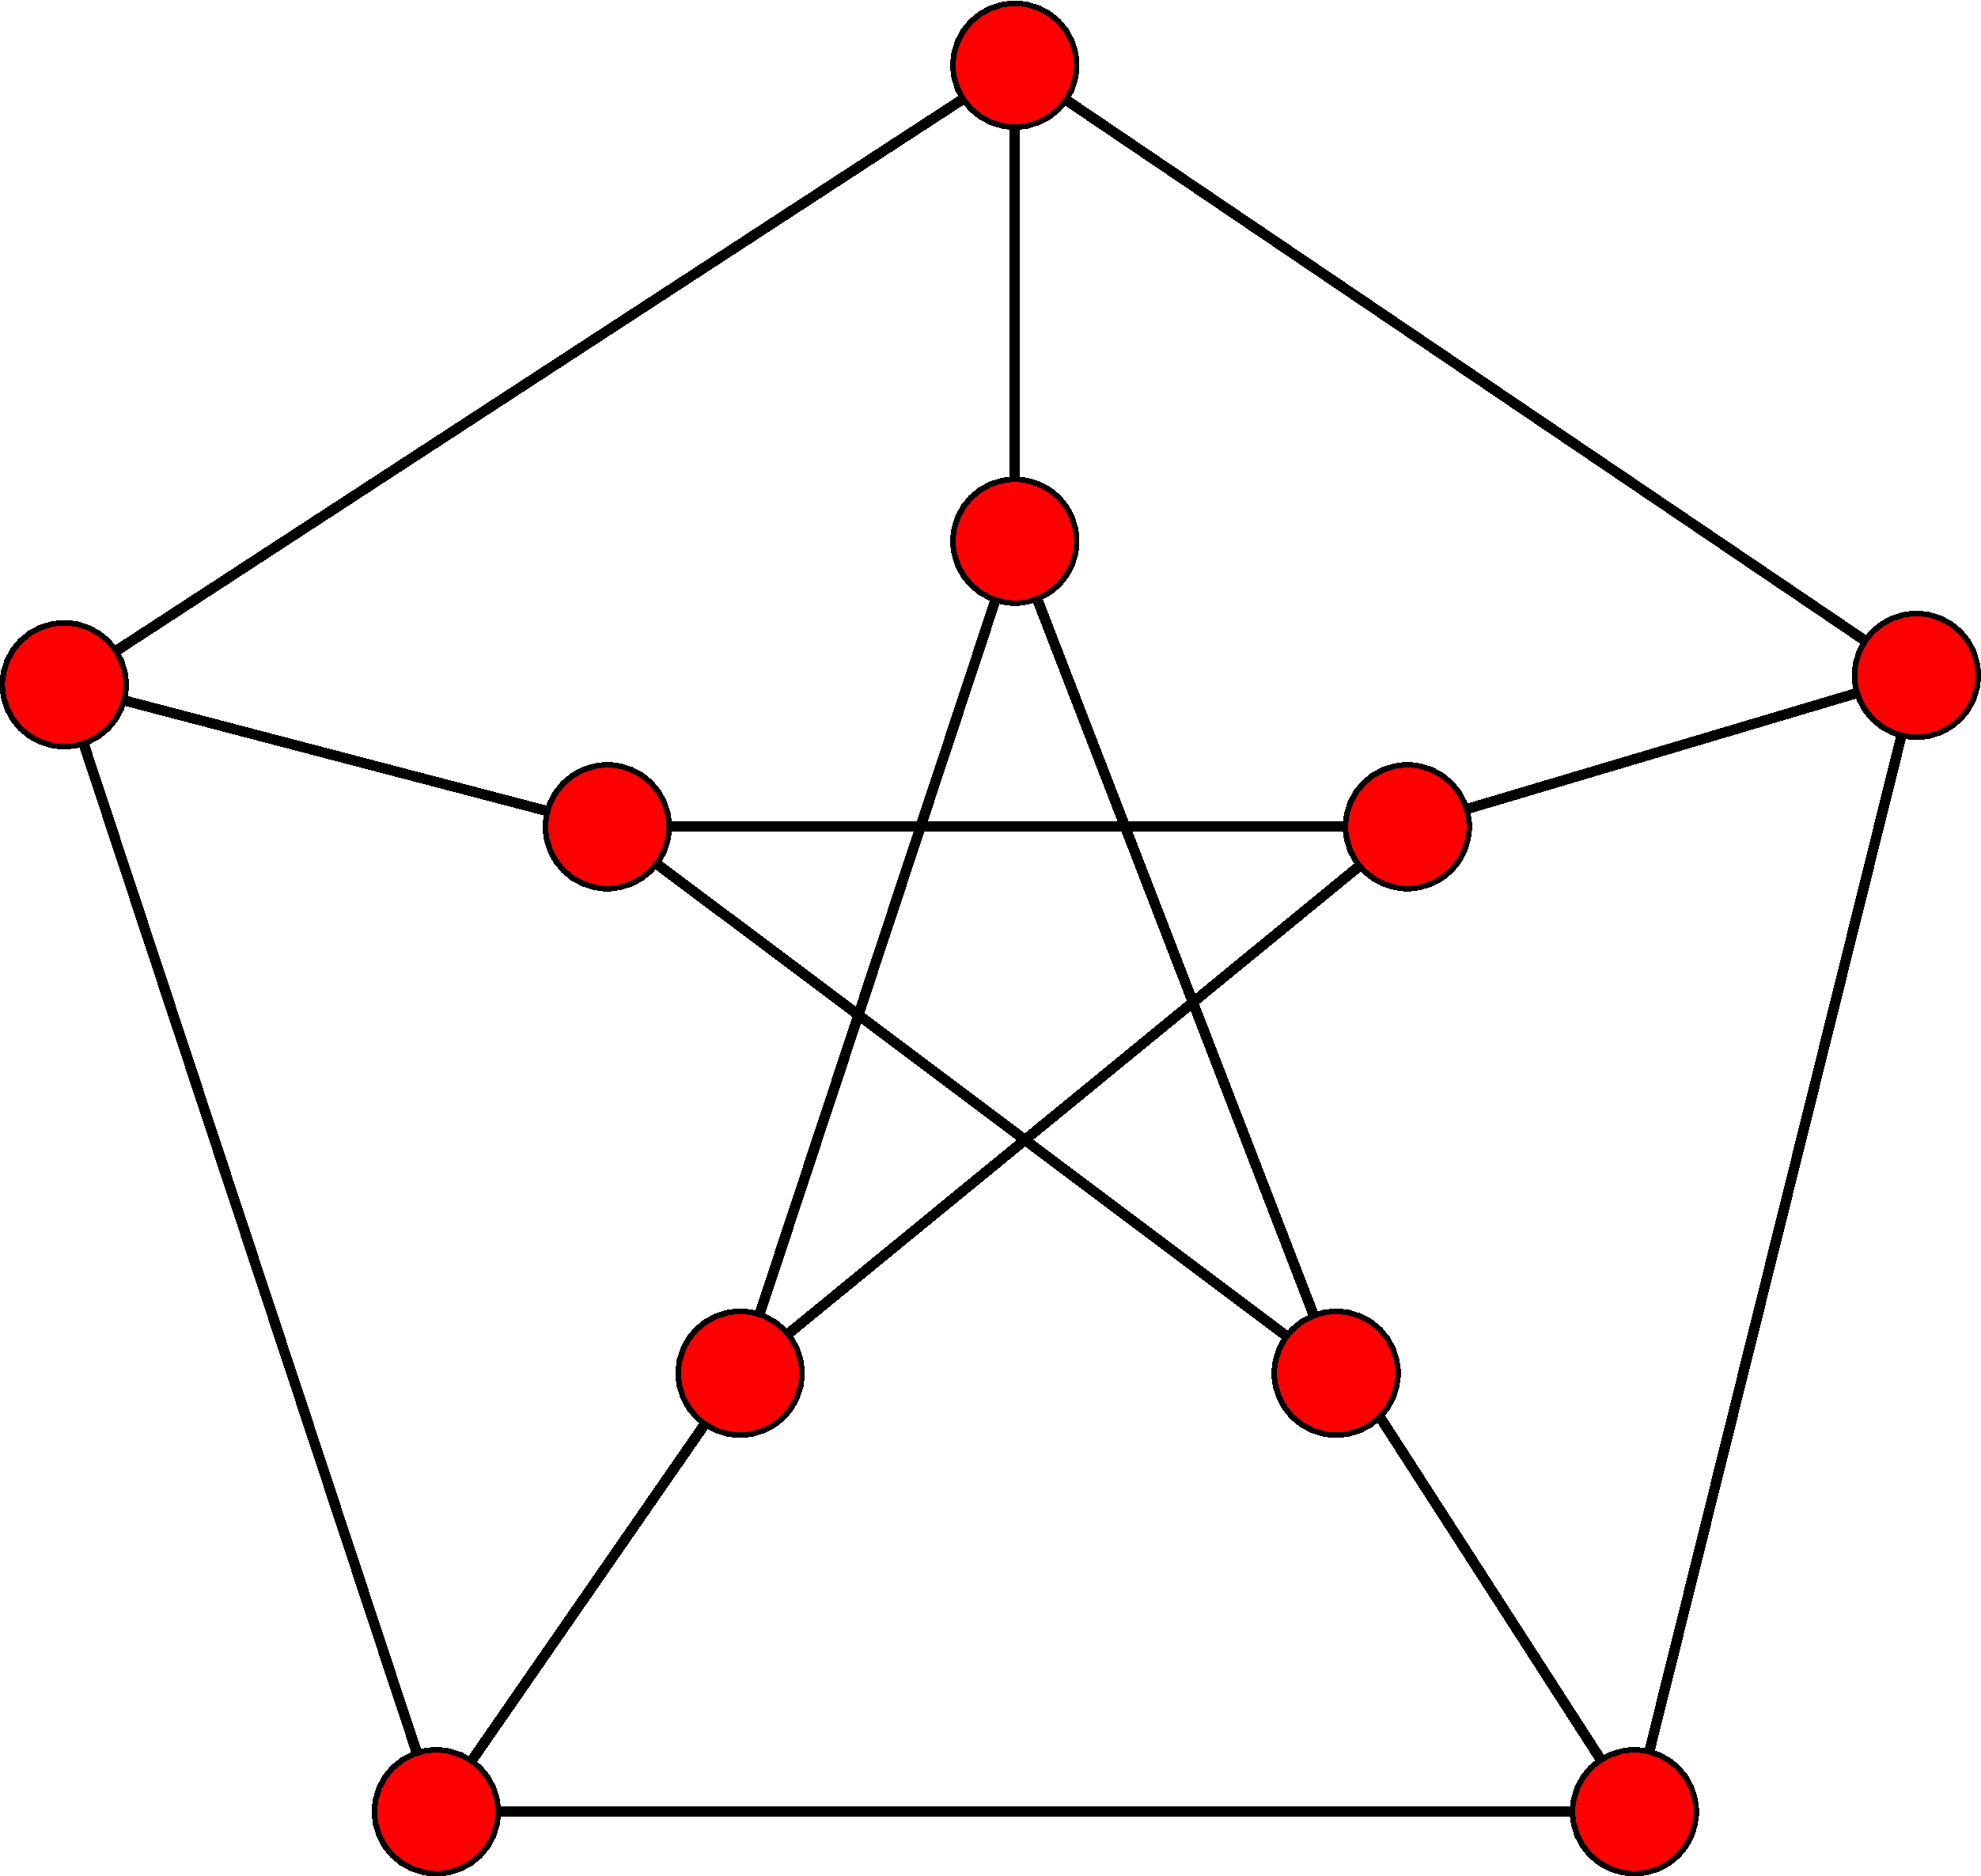
\includegraphics[keepaspectratio=true,width=\textwidth]{../planar-graphs/petersen-grundlage.pdf}
    \caption{Traditional realization of the Petersen graph as
    $KG_{5,2}$ in the plane. The inner vertices and their edges form a
    pentagram; the outer vertices form a pentagon. This version
    exhibits five edge intersections.}
    \label{fig:petersen}
  \end{subfigure}\hfill
  \begin{subfigure}[t]{.45\textwidth}
    \centering
    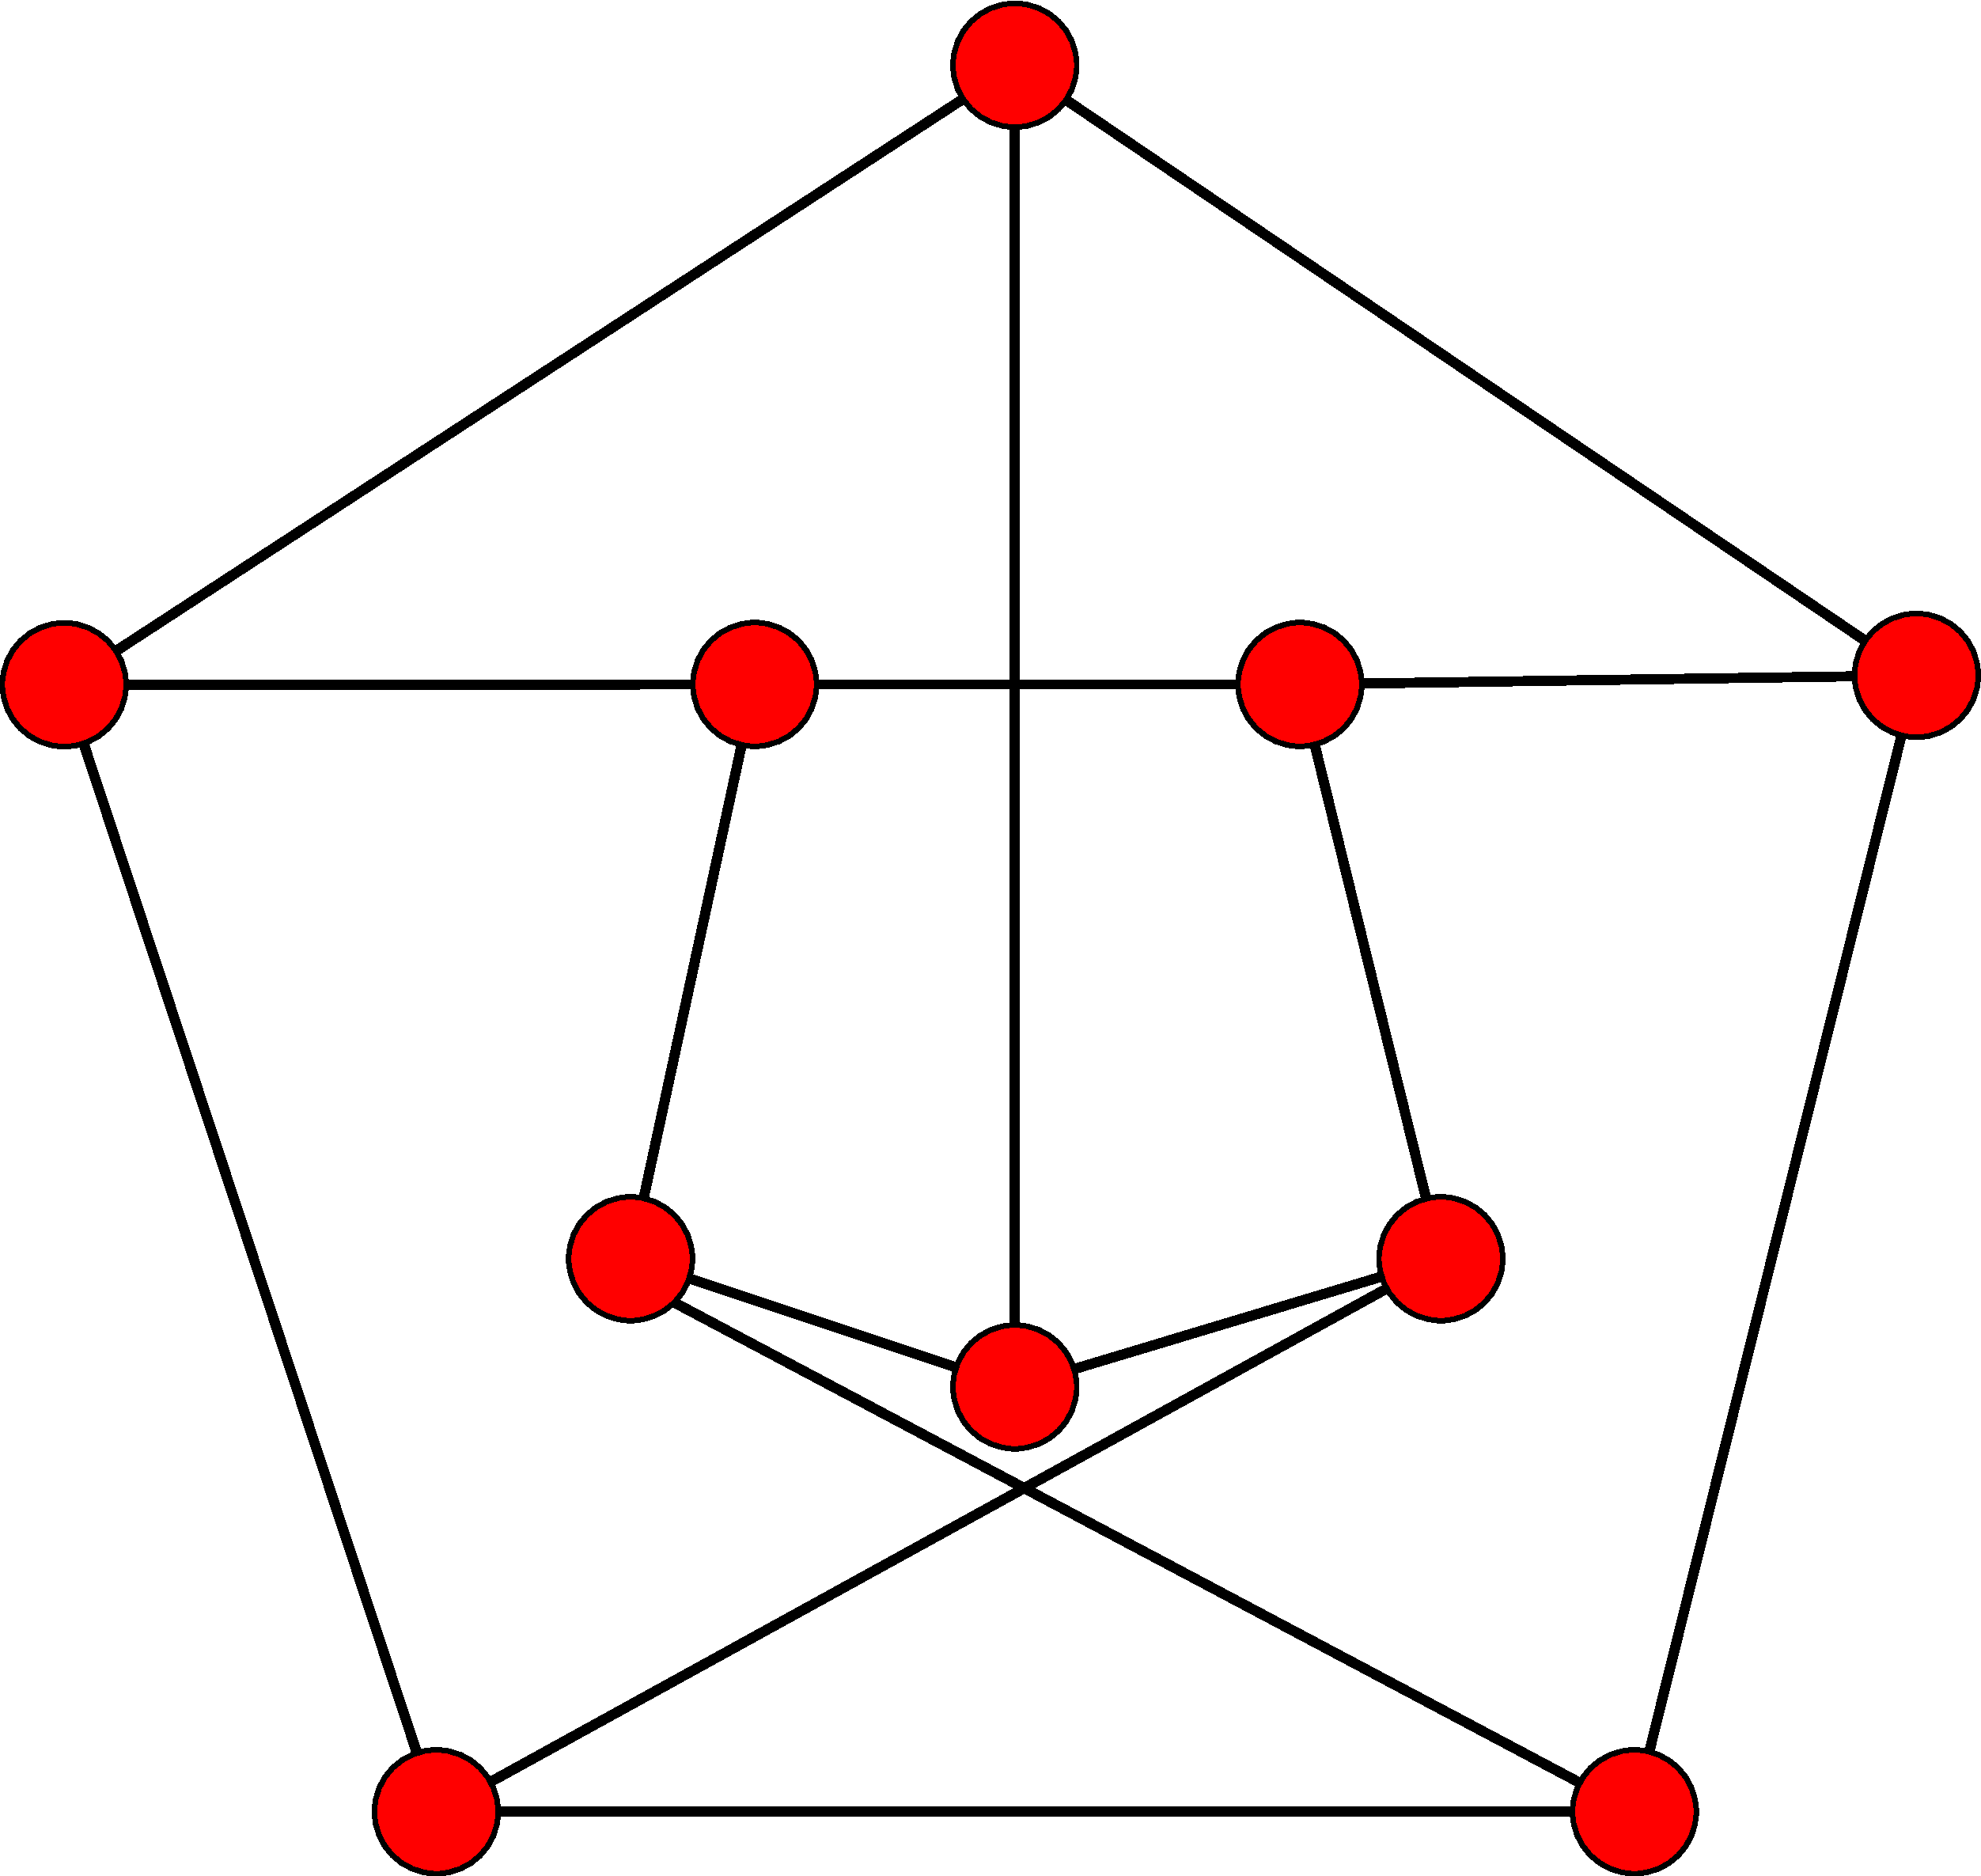
\includegraphics[keepaspectratio=true,width=\textwidth]{../planar-graphs/petersen-zweikreuzungen.pdf}
    \caption{The Petersen graph in the plane with just two edge
      intersections. It can be shown that this is the minimum number of
      intersections necessary when drawing the graph in the plane.}
    \label{fig:petersen-twointersect}
  \end{subfigure}
  \caption{Two drawings of the Petersen graph in the plane}
\end{figure}

The Petersen graph has the following interesting properties \cite{petersengraphbook,petersen}:

\begin{itemize}
  \item It has chromatic number $n - 2k + 2 = 3$, so an optimal vertex
    coloring needs at least three different colors (see figure
    \ref{fig:color-vertex})
  \item It has chromatic index 4, meaning a minimum edge coloring must
    use at least four different colors (see \ref{fig:color-edge})
  \item It is the smallest \emph{snark}\footnotemark[1]{} -- a
    connected, bridgeless\footnotemark[2]{}, 3-regular graph with chromatic index 4
    \footnotetext[1]{Julius Petersen constructed this graph in order to show
    that not all connected, bridgeless cubic graphs have chromatic
    index 3. In fact the Petersen graph, constructed in 1898 by
    Petersen, remained the only known counterexample until 1946
    (cf.~\cite[p.~71]{petersengraphbook}).}%
    \footnotetext[2]{Removing an arbitrary edge will not break the
    connectedness of the graph.}
  \item It has crossing number $\operatorname{cr}(P) = 2$,
    meaning it cannot be embedded into the Euclidean plane
    $\mathbb{R}^2$  with less than 2 edge intersections
    (cf.~\cite[p.~2]{crossingnr}, see figure~%
    \ref{fig:petersen-twointersect}).
\end{itemize}

The Petersen graph can, however, be embedded without any edge
intersections in the real projective plane, a model of which is the
cross cap.
While there are intuitive visualizations in the Euclidean plane for
the graph-theoretical properties, the embedding on the cross cap
should be done in a 3D setting. This will be done in
section~\ref{sec:maya}.

\begin{figure}[p]
  \begin{subfigure}[t]{.45\textwidth}
    \centering
    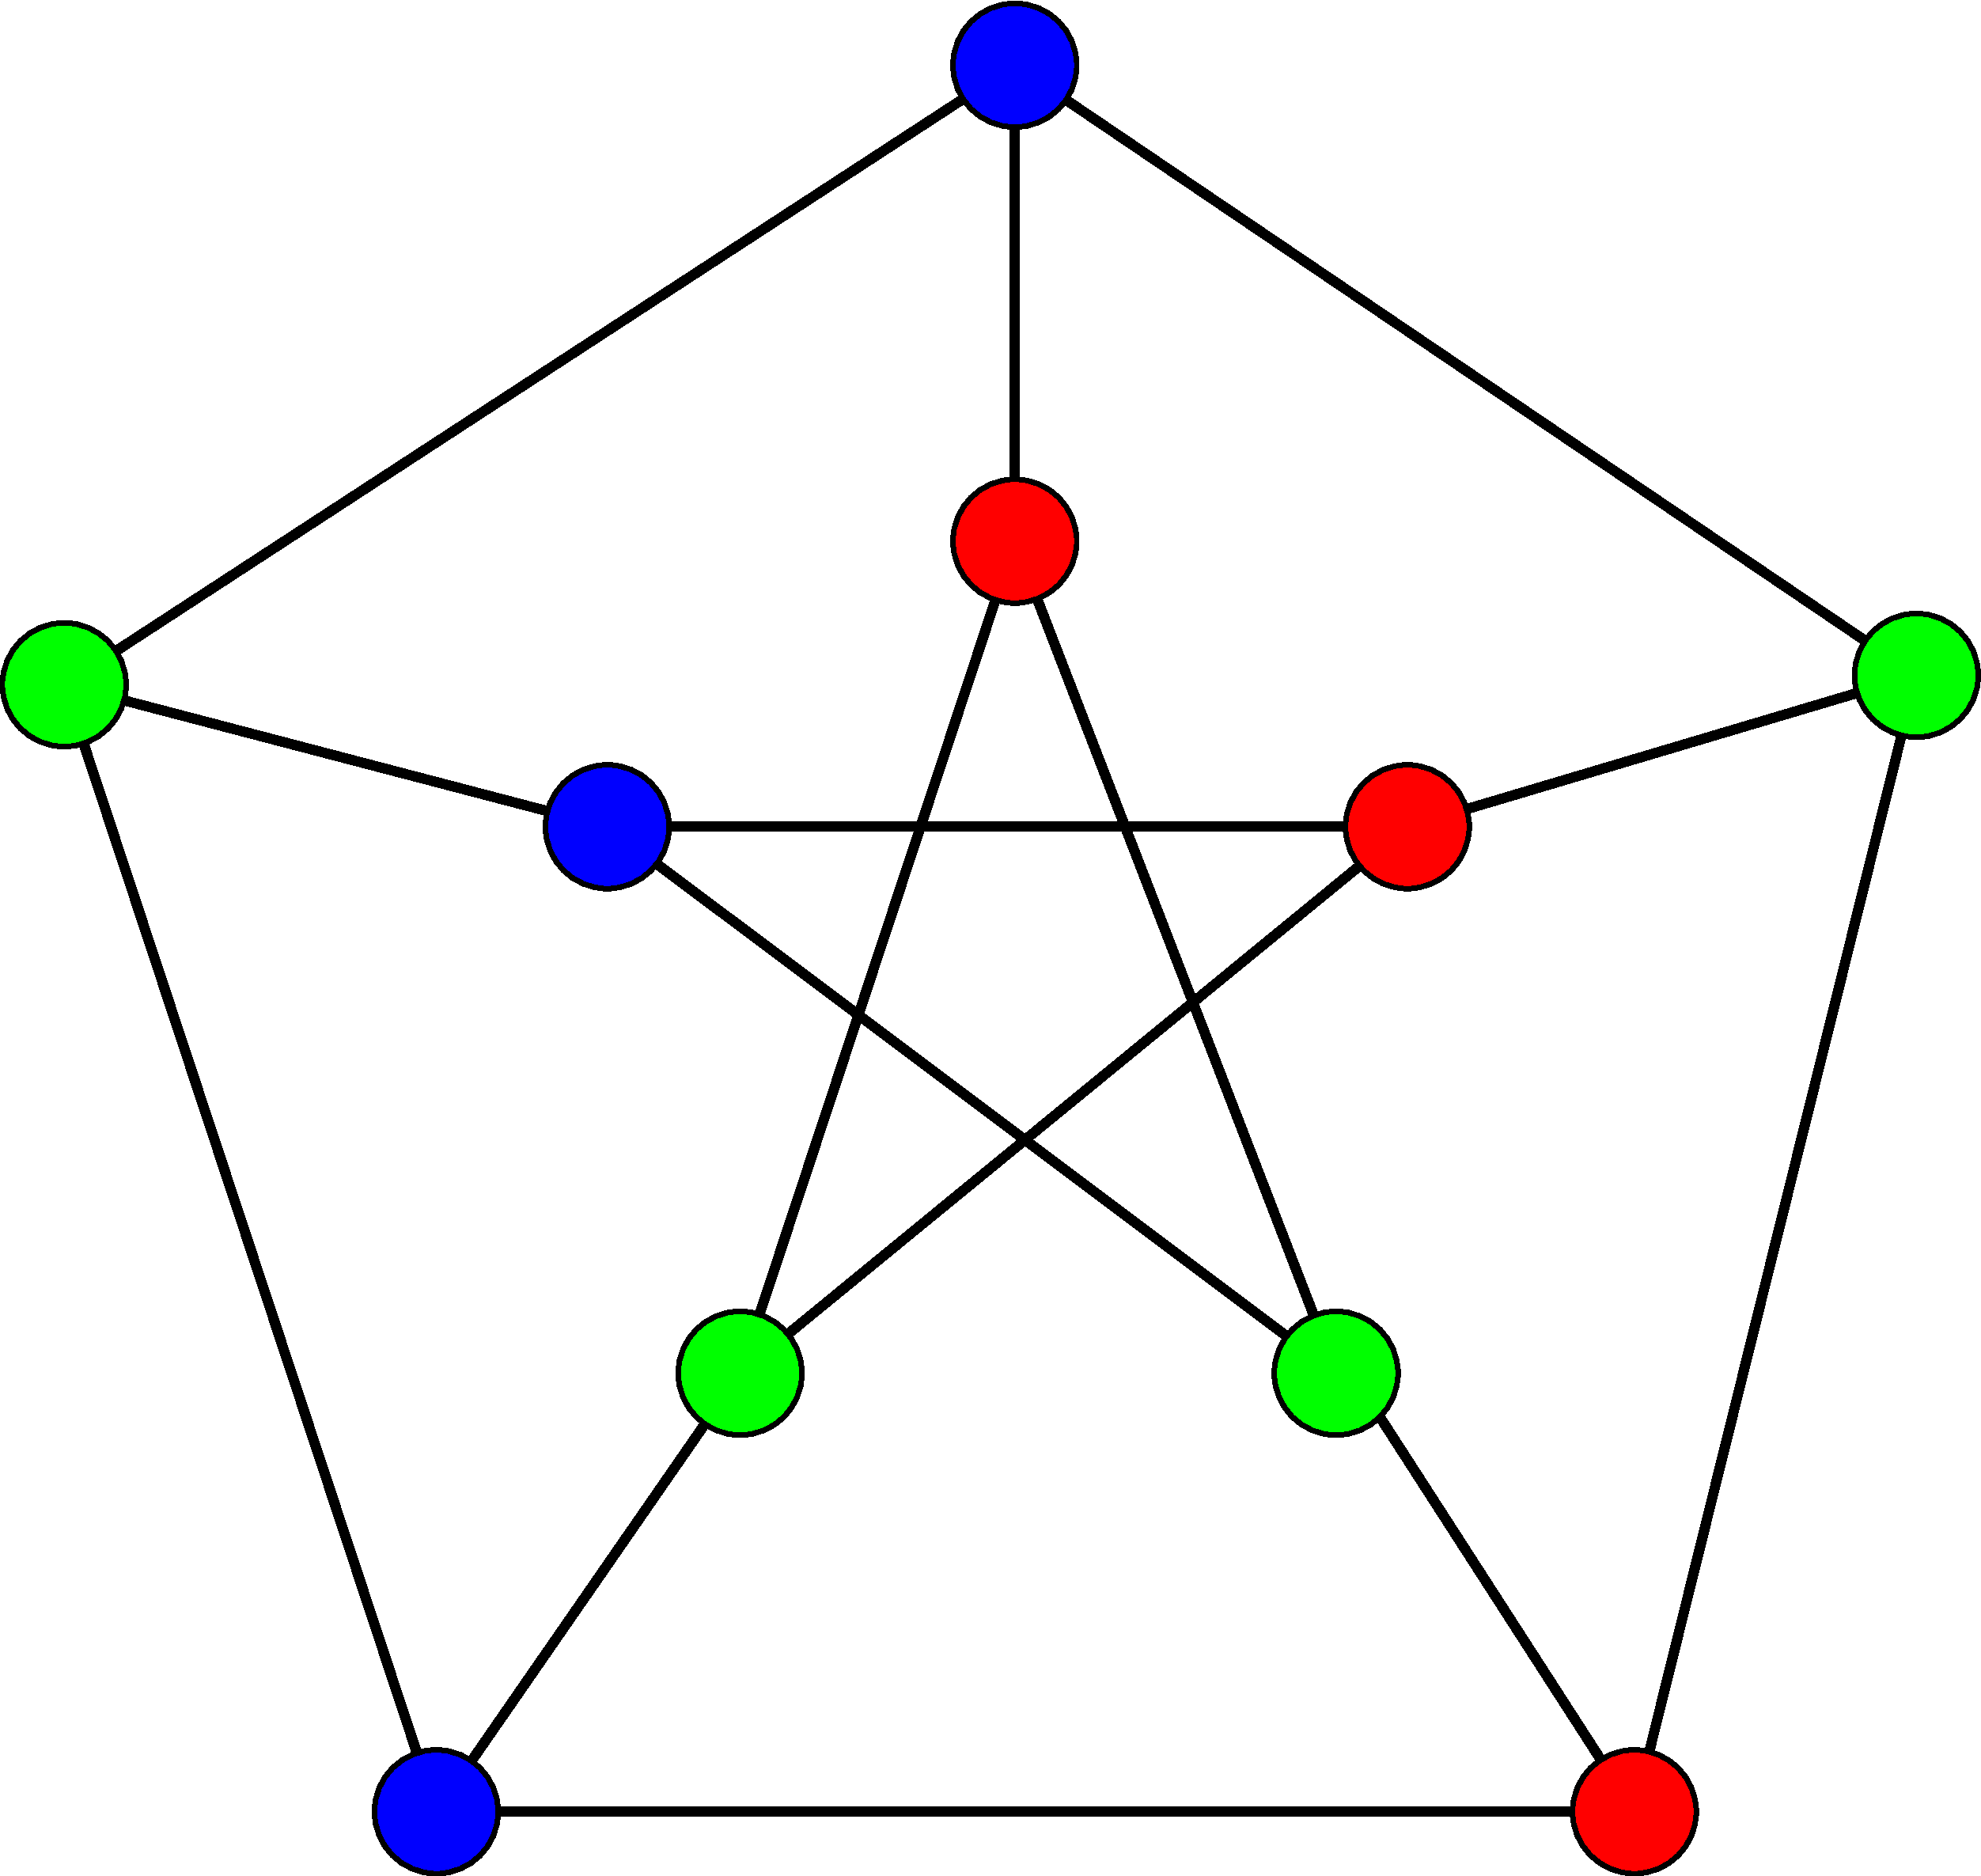
\includegraphics[keepaspectratio=true,width=\textwidth]{../planar-graphs/petersen-vertex-threecoloring.pdf}
    \caption{A vertex 3-coloring of the Petersen graph}
    \label{fig:color-vertex}
  \end{subfigure}\hfill
  \begin{subfigure}[t]{.45\textwidth}
    \centering
    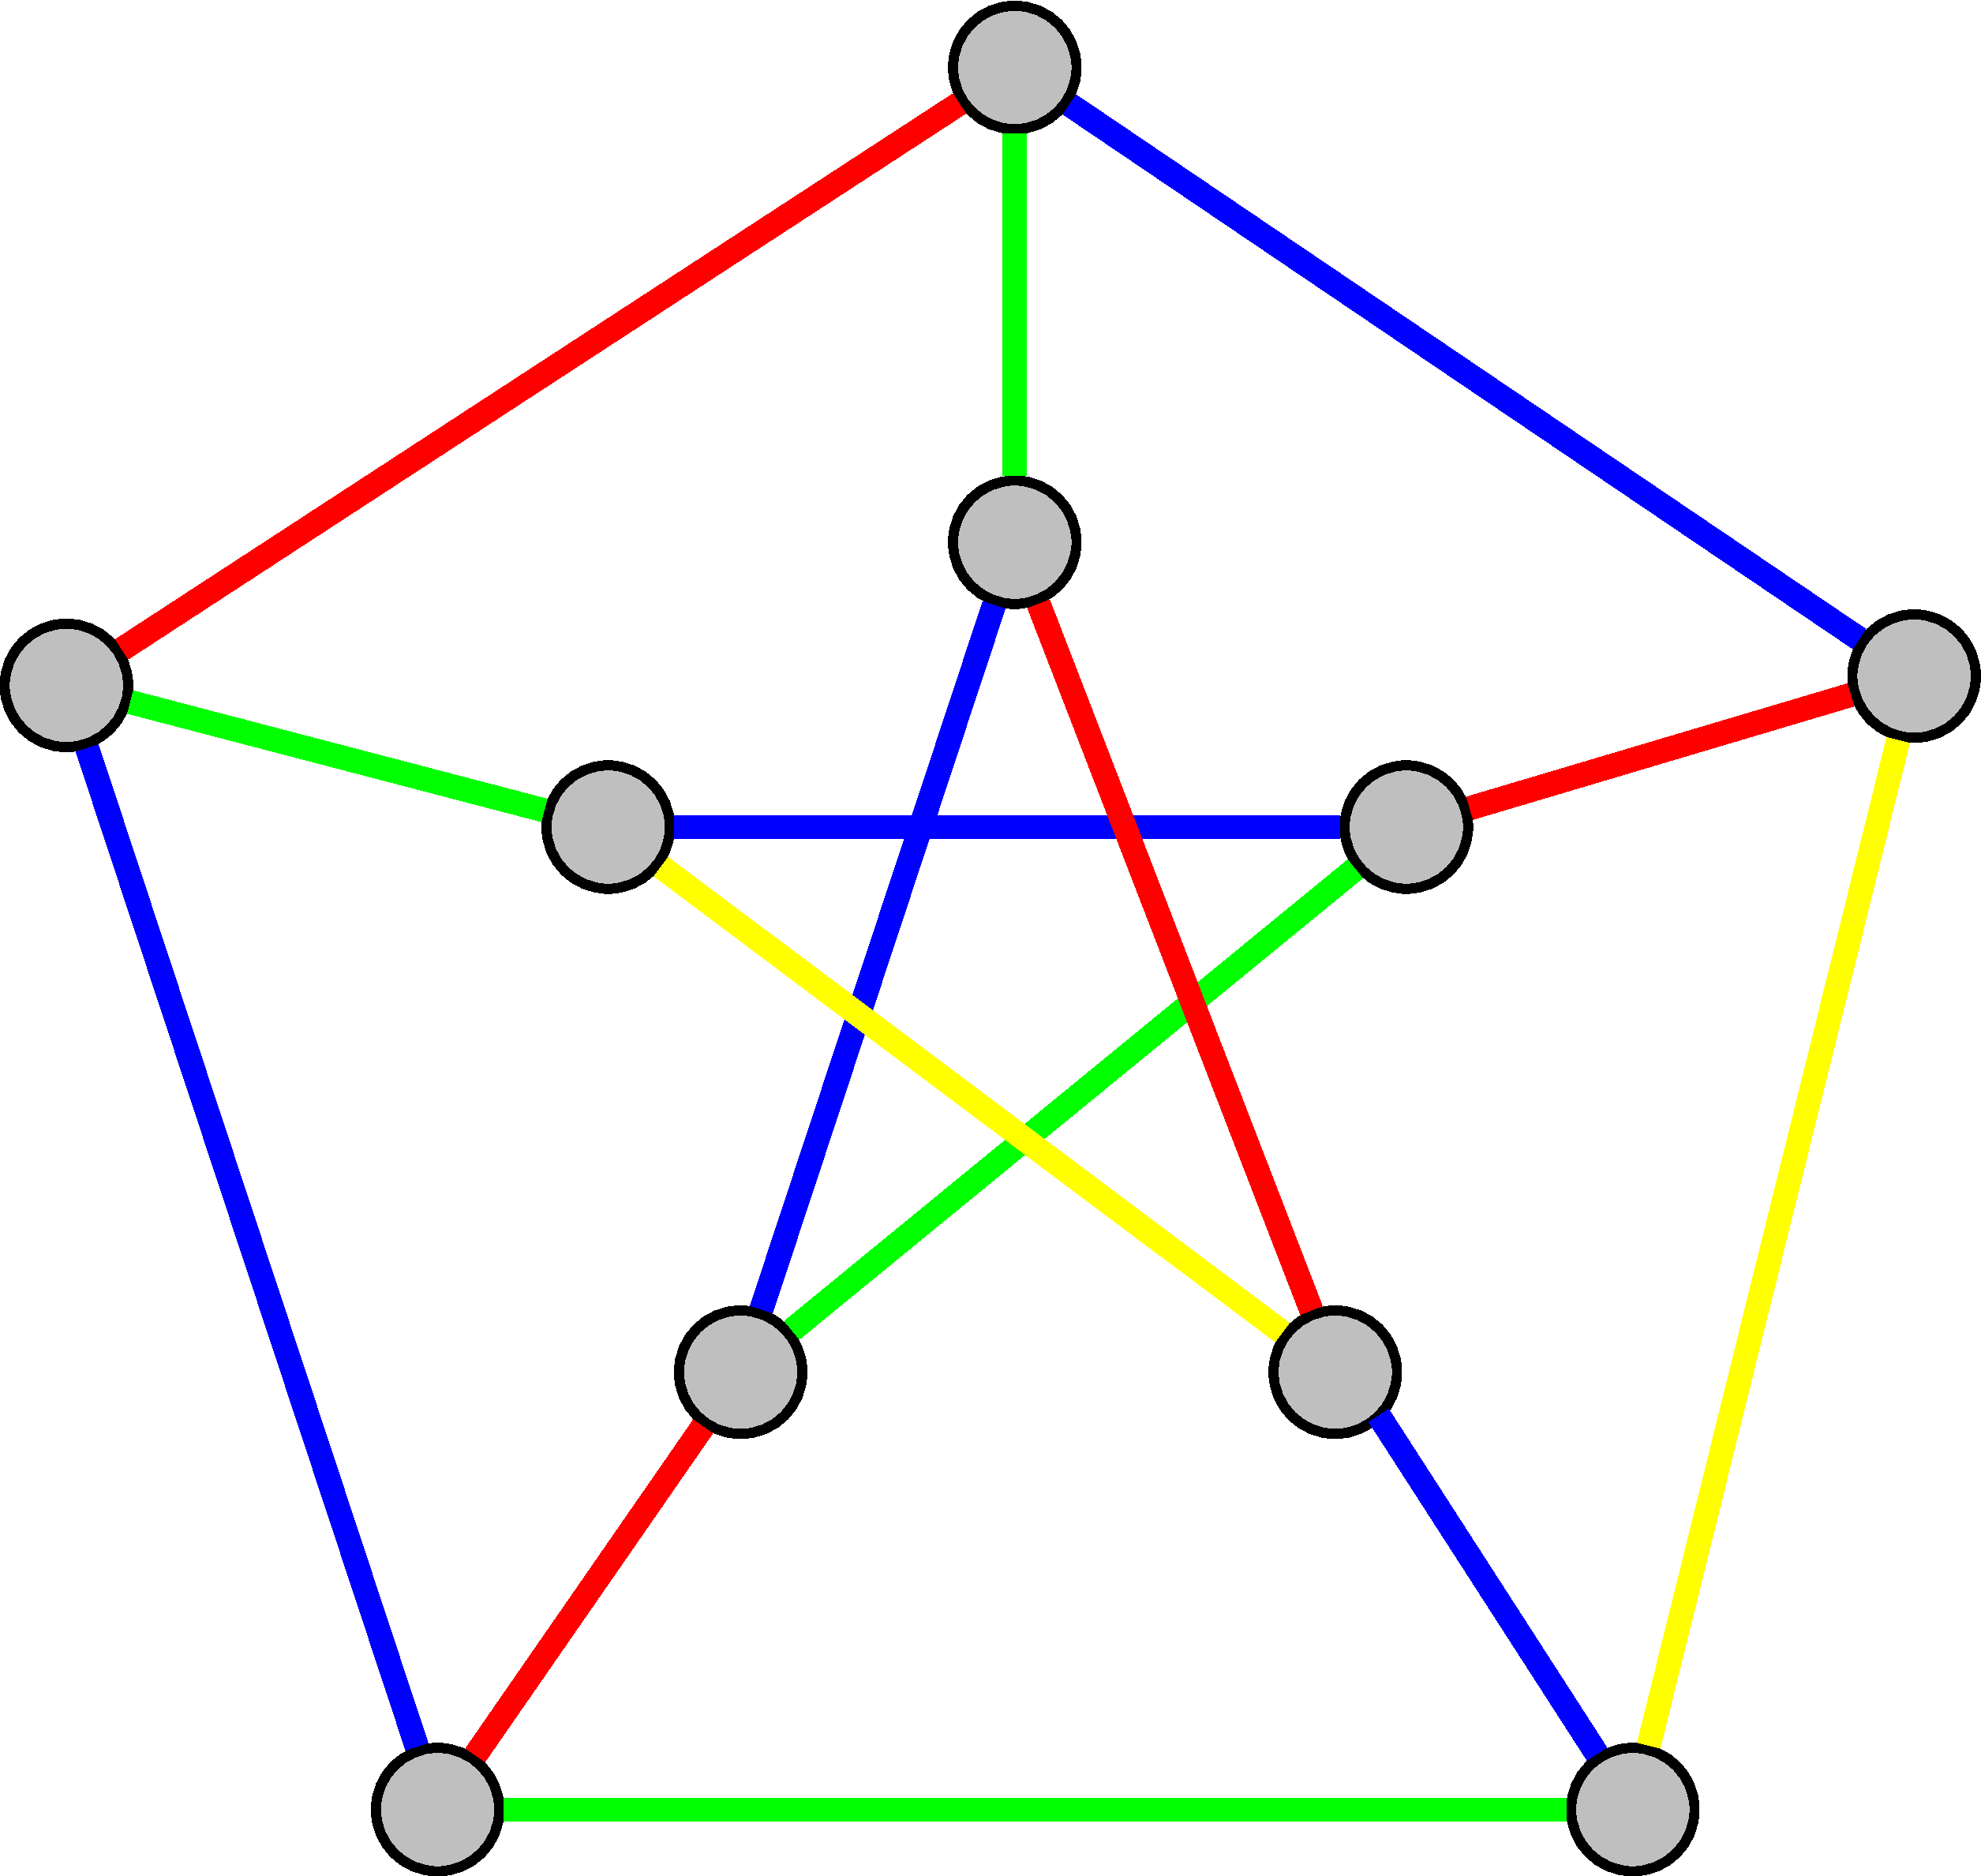
\includegraphics[keepaspectratio=true,width=\textwidth]{../planar-graphs/petersen-edge-fourcoloring.pdf}
    \caption{An edge 4-coloring of the Petersen graph}
    \label{fig:color-edge}
  \end{subfigure}
  \caption{The Petersen graph has chromatic number 3 and chromatic index 4}
\end{figure}

\subsection{The Real Projective Plane and the Cross Cap}
\label{sec:rp2}

\begin{definition}[Real projective space]
  The \emph{real projective space} $\mathbb{R}P^n$ consists of the lines
  passing through the origin of $\mathbb{R}^{n+1}$. In the case $n=1$,
  this is called the \emph{real projective line}; in the case $n=2$,
  \emph{real projective plane}.
\end{definition}
%
\begin{minipage}[t]{0.57\textwidth}
  An equivalent (and more intuitive) construction for $\mathbb{R}P^n$
  can be given by identifying antipodal points of the $n$-sphere $S^n$: Since any
  line passing through the origin meets the sphere at exactly two
  antipodal points, one can identify a line by either of these points.
  Choosing w.\,l.\,o.\,g.~the points on the northern hemisphere,
  one finds that the real projective plane is topologically equivalent to
  the disk $D^2$ with antipodal points of the border $\partial D^2 =
  S^1$ identified.\\[1em]
  Stretching the imagination a little bit, we can picture $D^2$ as the
  topologically equivalent unit square. The identification of
  antipodal border points then happens as in figure \ref{fig:rp2}.
\end{minipage}%
\hfill%
\begin{minipage}[t]{0.35\textwidth}
  \vspace{-.7cm}%
  \begin{figure}[H]
    \centering
    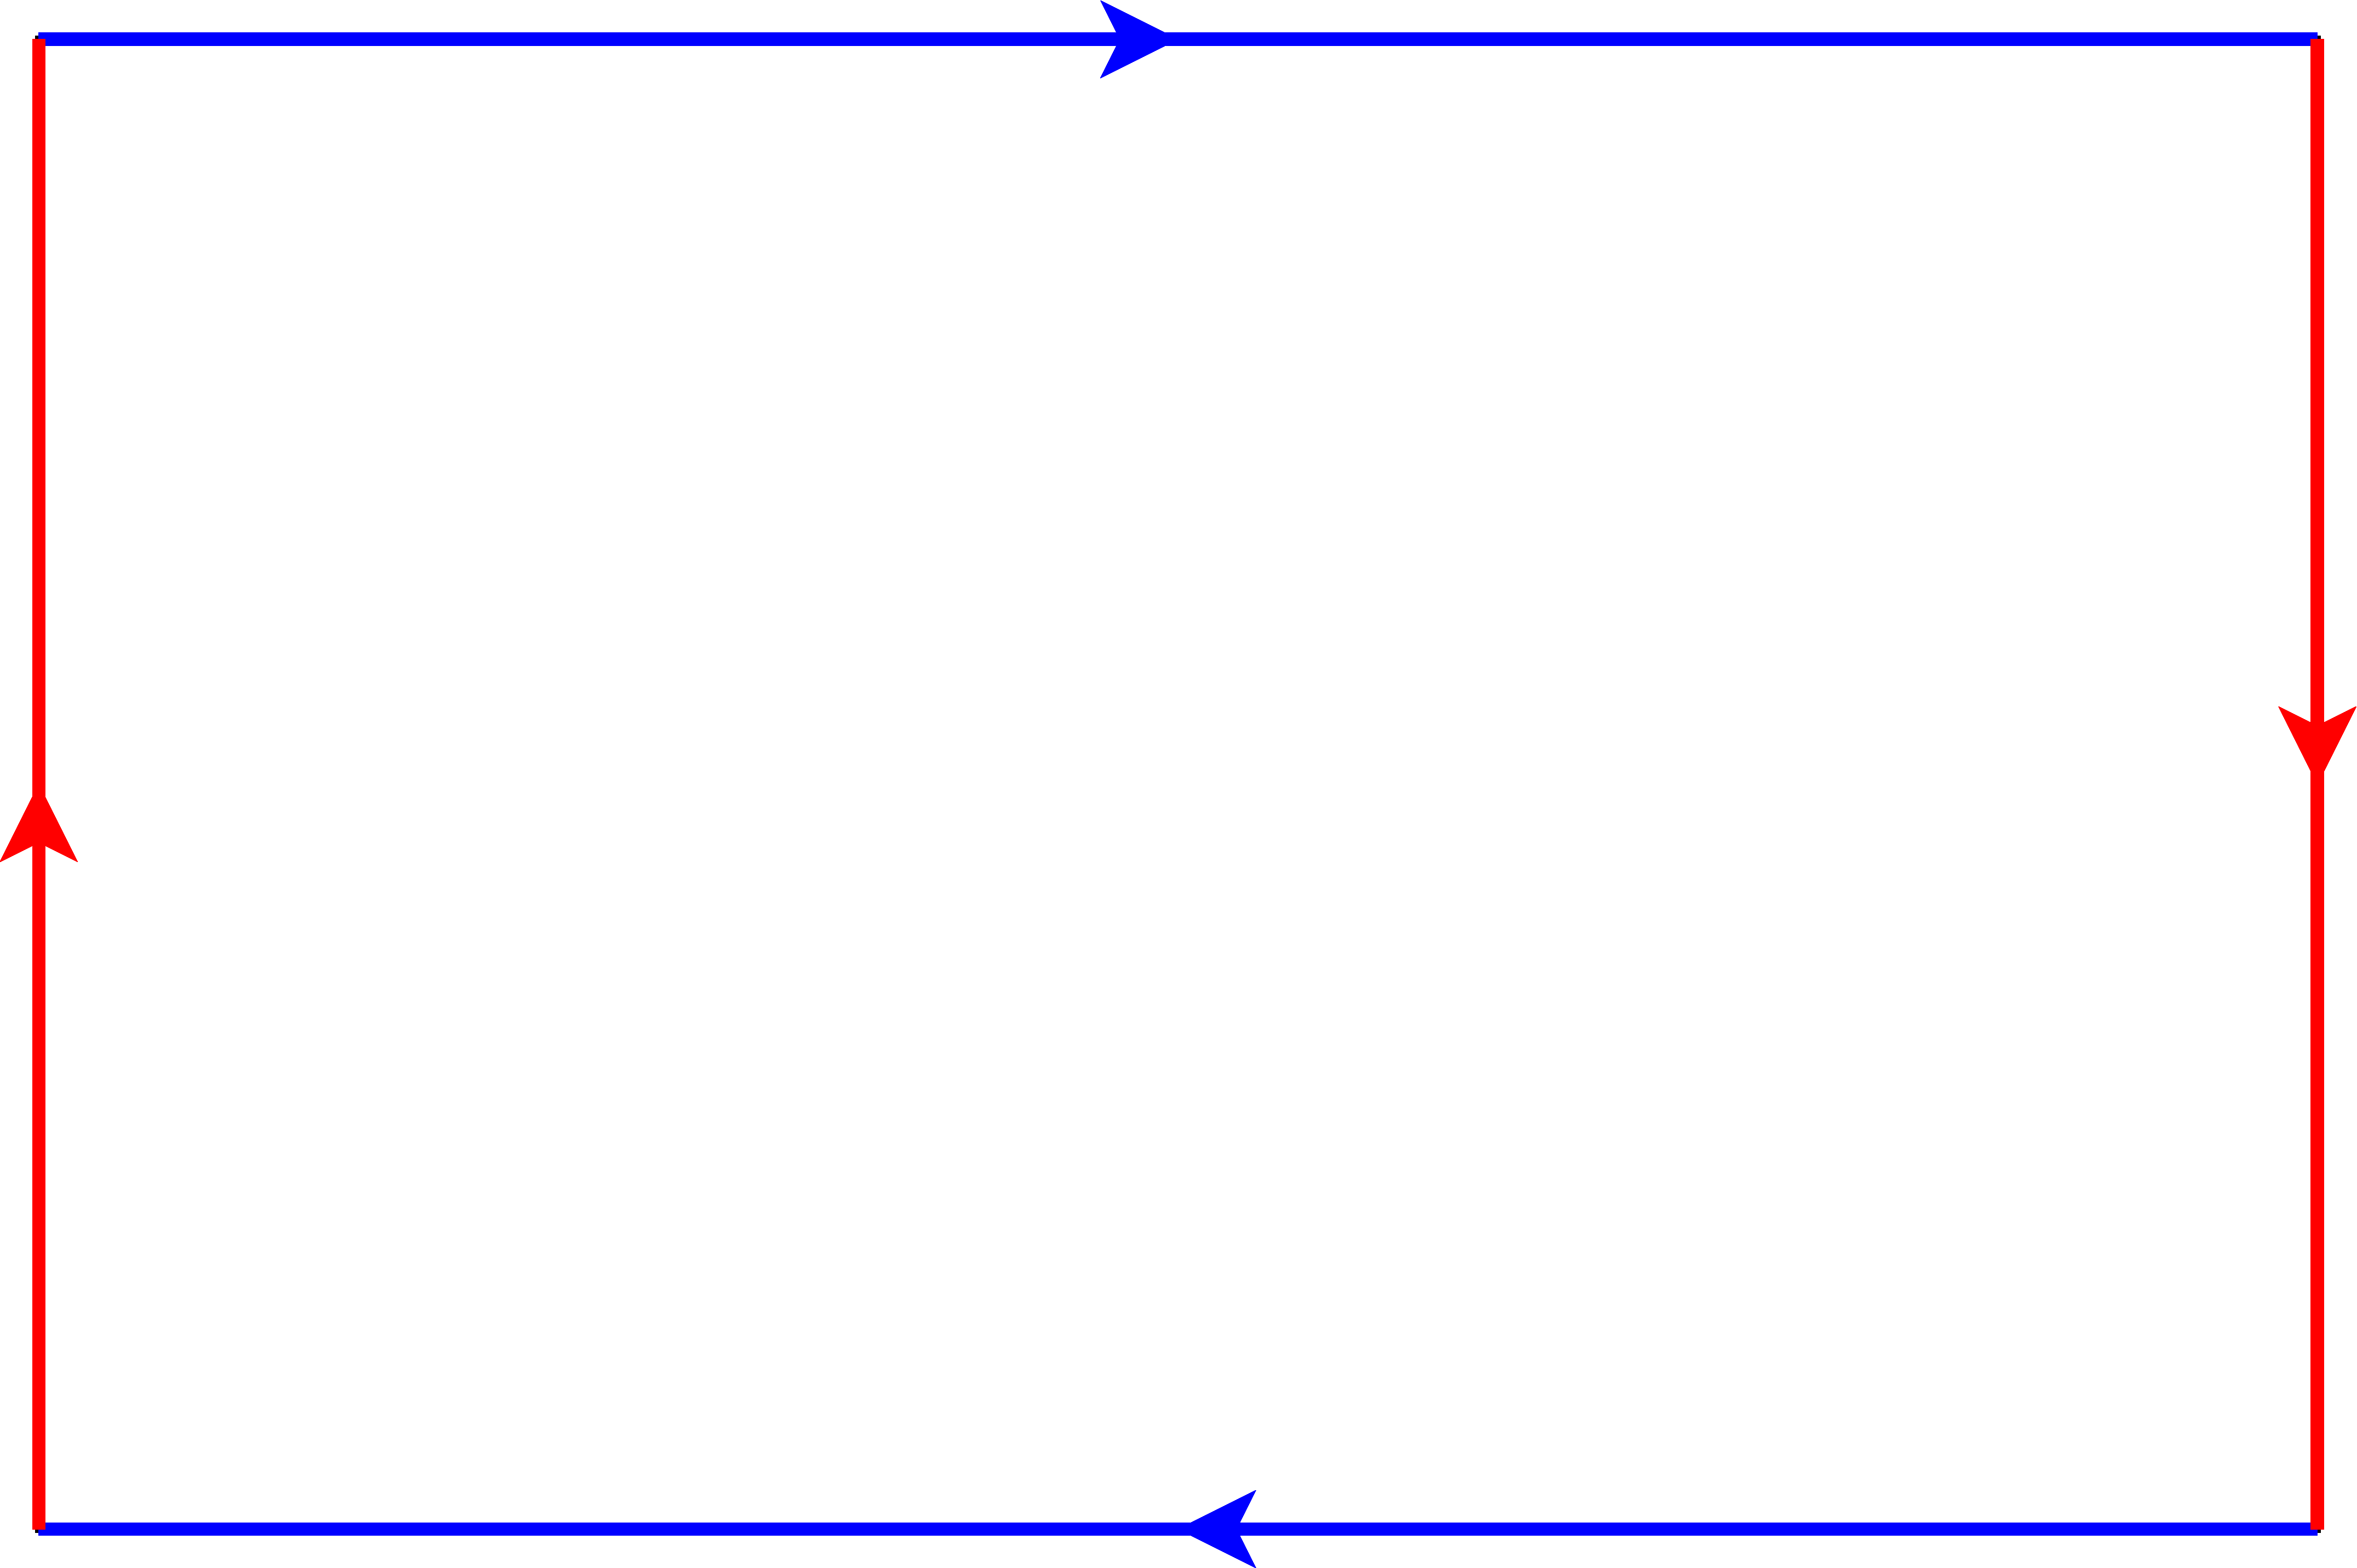
\includegraphics[keepaspectratio=true,width=\textwidth]{../planar-graphs/crosscap-construction.pdf}
    \caption{The topological view: How to glue $[0,1]\times[0,1]$
      together to construct the real projective plane.}
    \label{fig:rp2}
  \end{figure}
\end{minipage}%

The homology of $\mathbb{R}P^n$ is \cite[2.42]{hatcher}:
\[
  H_k(\mathbb{R}P^n;\;\mathbb{Z}) =
                   \begin{cases}
                      \mathbb{Z} & \text{if }k = 0\text{ or }k = n\text{ odd} \\
                      \mathbb{Z}/2\mathbb{Z} & \text{if $k$ odd and } 0 < k < n \\
                      0 & \text{otherwise} \\
                   \end{cases}
\]
As a corollary of the Alexander duality \cite[3.45]{hatcher}, any compact and locally
contractible subspace of $\mathbb{R}^n$ is torsion-free in homology of
degree $n-2$. But $H_1(\mathbb{R}P^2;\;\mathbb{Z}) = \mathbb{Z}/2\mathbb{Z}$, hence
the real projective plane cannot be embedded into $\mathbb{R}^3$; it
can only be \emph{immersed}, i.\,e.~it can be locally embedded at any
point.

The \emph{cross cap} is a two-dimensional real manifold that is
homeomorphic to the real projective plane $\mathbb{R}P^2$. It will
serve as our model of the real projective plane in $\mathbb{R}^3$.

\subsection{Embedding the Petersen Graph on the Cross Cap}
\label{sec:rp2embedding}

Using this “planar model” of $\mathbb{R}P^2$, we can now easily see
that an embedding of the Petersen graph without edge intersection onto
the surface of the cross cap is in fact possible.
To see this, start with the Petersen graph in the form with just two
edge intersections (figure \ref{fig:petersen-twointersect}), leaving
out all the edges that would intersect.
Embedded in $\mathbb{R}P^2$ (figure \ref{fig:rp2}) one now draws the
remaining edges in the following fashion, taking the orange line as an
example (cf. figure \ref{fig:rp2embedding}):
Draw the edge to leave the $[0,1]\times[0,1]$ square (with origin at
the lower left, say) at $(0,\,1/4)$.
Because the red sides are glued together with opposite orientation,
continuing to draw this edge will commence from $(1,\,3/4)$.
In the same fashion, the green edge passes the points $(0,\,3/4)$ and
$(1,\,1/4)$ simultaneously (because they are in fact the same point in
this construction); the same goes for the black line at the points
$(0,\,1/2)$ and $(1,\,1/2)$.
Neither of these points induce a crossing.

\begin{figure}[h]
  \centering
  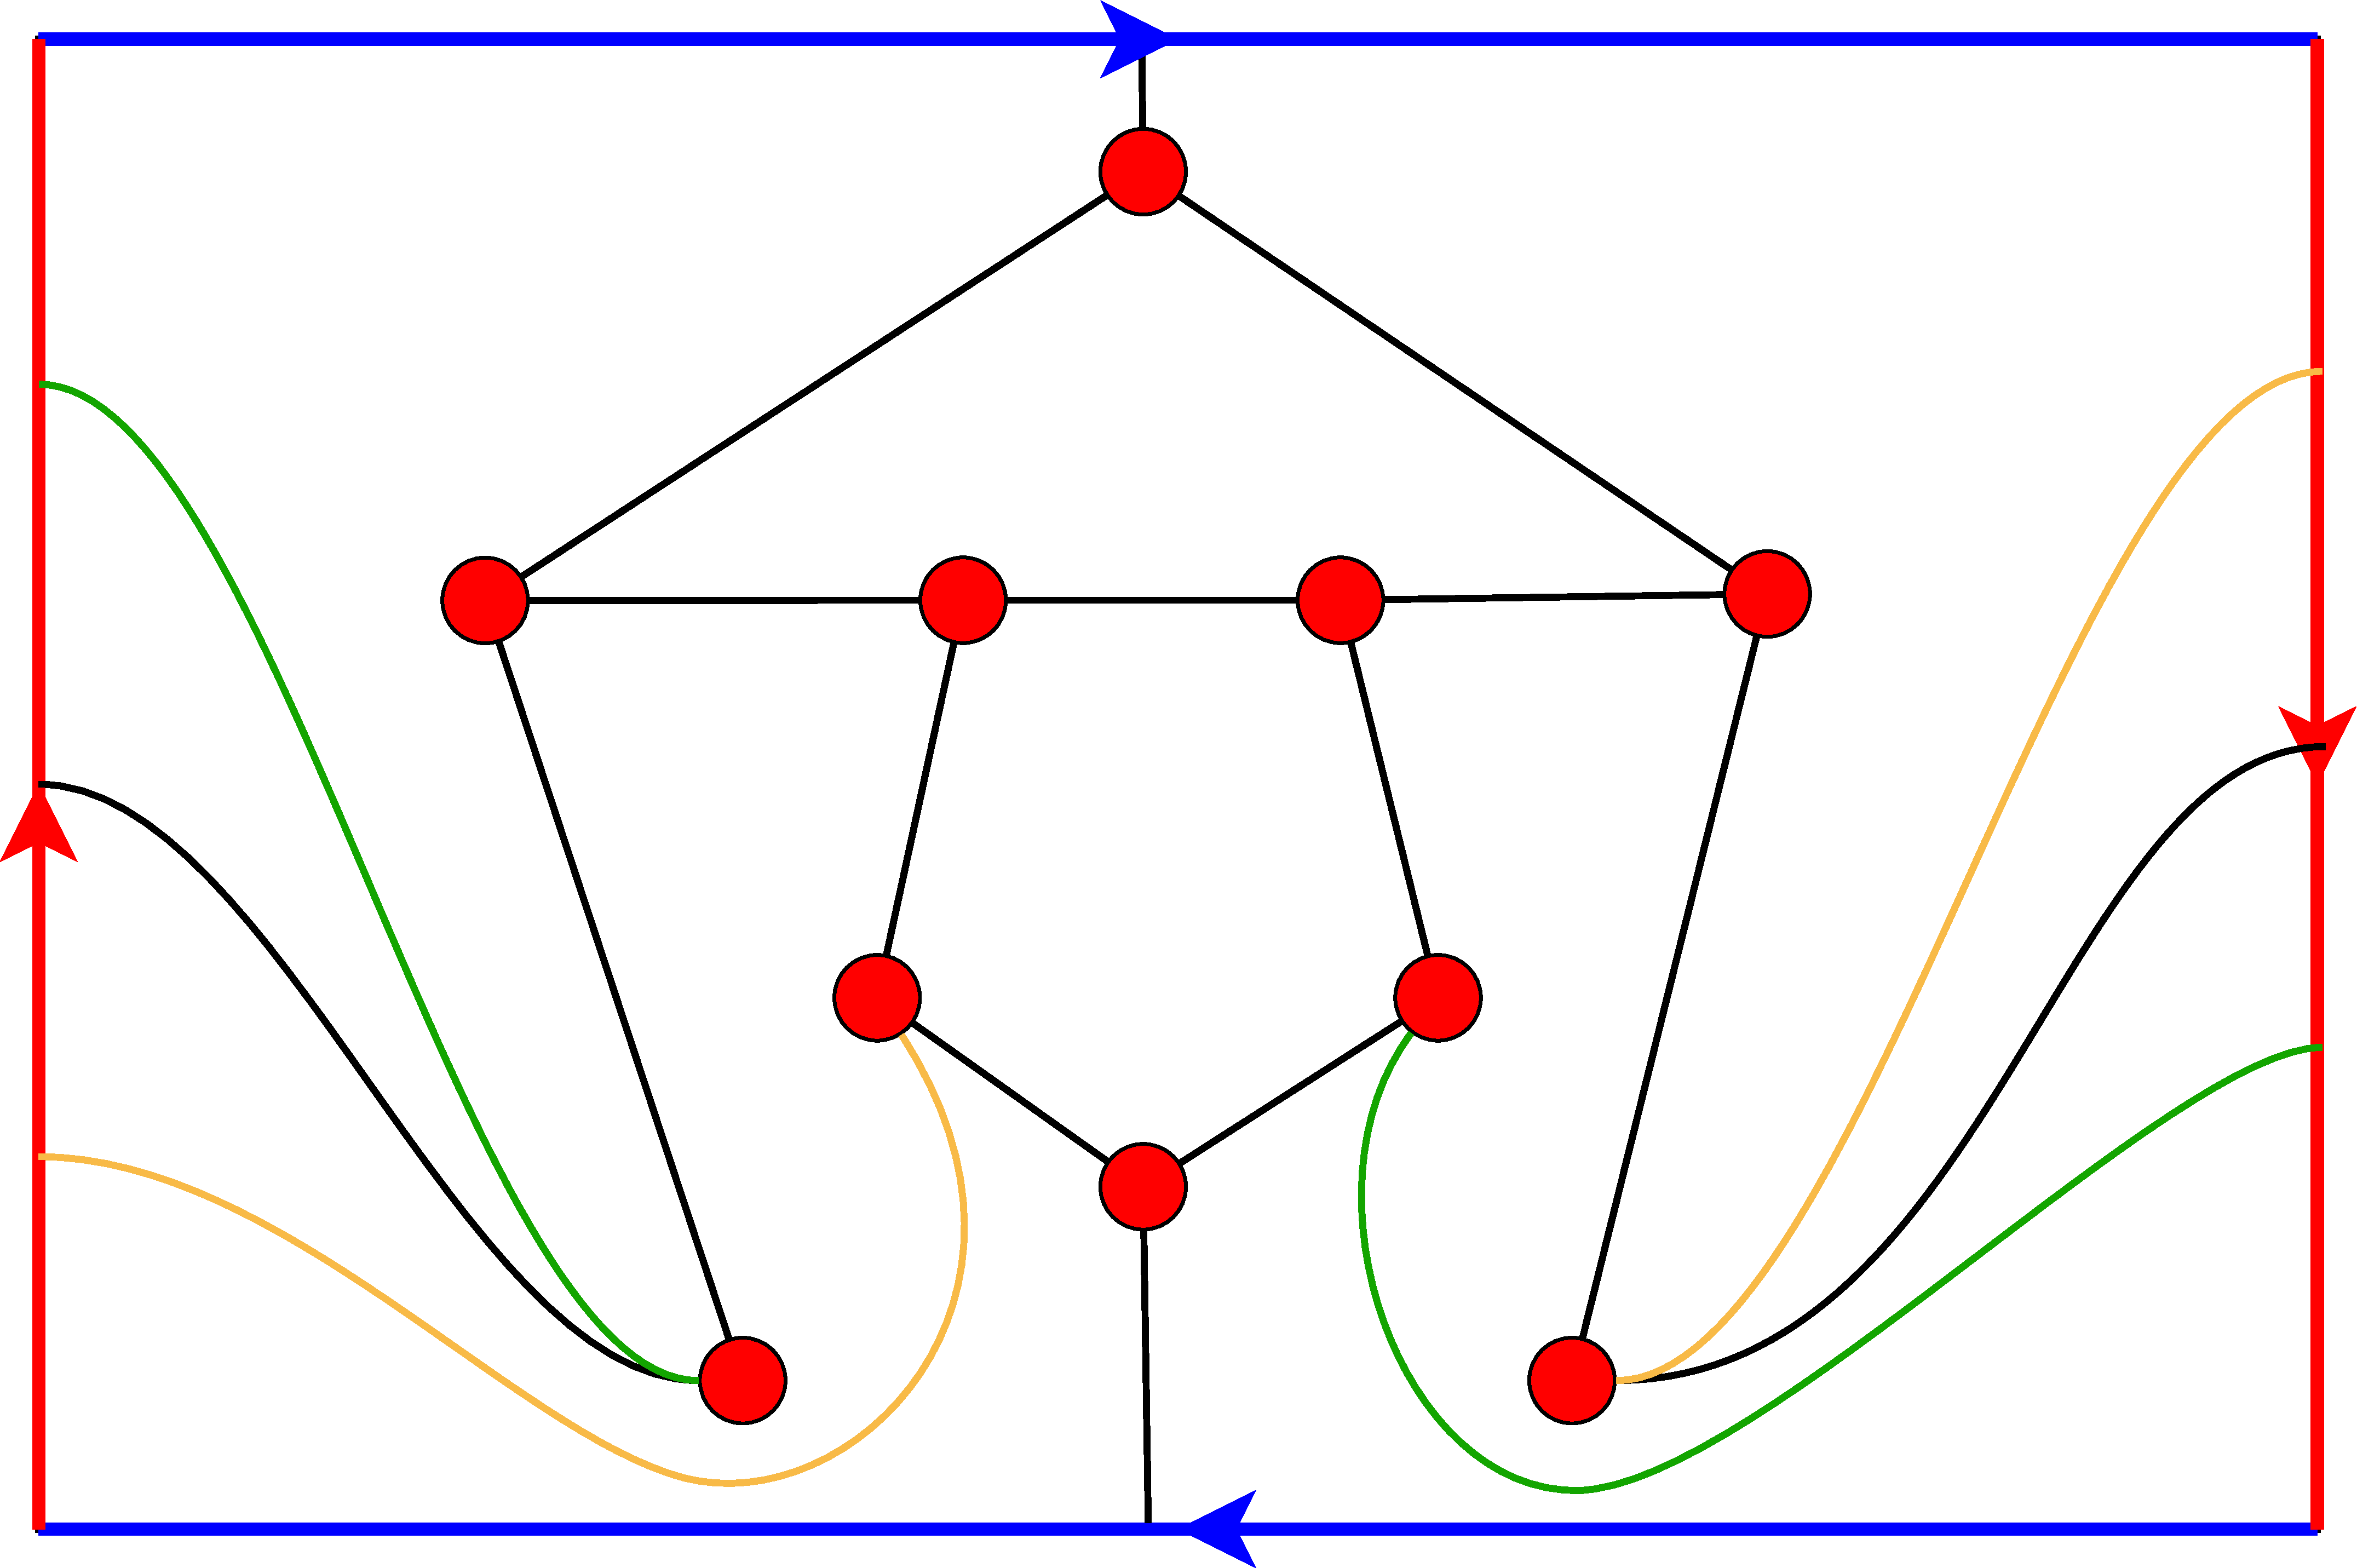
\includegraphics[keepaspectratio=true,width=0.7\textwidth]{../planar-graphs/crosscap-embedding-5.pdf}
  \caption{An embedding of the Petersen graph without edge
    intersection on the surface of the cross cap.}
  \label{fig:rp2embedding}
\end{figure}

This result shows that it is in fact possible to embed the Petersen
graph onto the cross cap without any edge intersection -- however,
this model of the cross cap has hardly any resemblance of how a model
of it would look like immersed in $\mathbb{R}^3$.


\subsection{An Alternative Embedding Approach Using the Dodecahedron}
\label{sec:dodecahedron}

It is possible to obtain the embedding described in the previous
section along with a construction of the cross cap “in one step”. The
\emph{(regular) dodecahedron} (from gr.~\textgreek{δωδεκα}, twelve) is
the platonic solid that consists of 12 regular pentagonal faces. Three
of these faces meet at each vertex, hence the graph consisting of the
20 vertices and 30 edges is cubic.

One can now transfer the construction of $\mathbb{R}P^2$ from $S^2$ to
the dodecahedron: Identifying antipodal points, we get a surface that
consists of 6 faces and whose 10 vertices and 15 edges form the cubic
Petersen graph. While this construction is very neat and elegant, it
does not make clear how the Petersen graph appears on the surface.

\section{The \emph{Maya} Construction}
\label{sec:maya}

Given that it is hard to grasp the “actual look” of the cross cap
in its planar form, we realized it as a real 2-manifold embedded in
$\mathbb{R}^3$. To do this, we chose the 3D modeling software
\emph{Autodesk Maya\textregistered} (or simply \emph{Maya}). It is a state-of-the-art
system not only for modeling objects, but also for creating animations
with these objects.

Our goal was to create an insightful animation that highlights the
following points we previously outlined in section
\ref{sec:theoretical}:

\begin{itemize}
  \item How the cross cap can be immersed in Euclidean space $\mathbb{R}^3$
  \item How the immersion will have self-intersections
  \item How the Petersen graph can be embedded onto this surface
  \item How this embedding will not have edge intersections
\end{itemize}

In the following sections we will present our motivation for designing
the animation the way we did, and give a brief coverage of the
technical steps that were necessary in \emph{Maya} to produce this
result.

\subsection{Constructing the Cross Cap}

Initially we tried a construction of the cross cap starting with a
dodecahedron as outlined in section~\ref{sec:dodecahedron} and
motivated by \cite[p.~270f]{bilderbuch}.
A standard topological construction of point identification is
possible to achieve vertex or edge-wise:
Analogously to the construction of $\mathbb{R}P^2$ from $S^2$,
one can start off with one half of the dodecahedron and continue to
identify border edges and vertices, bending and inflating the object
in the process.
The advantage of this process is that it is producing the Petersen
graph “for free” from the original edges.

This construction process works well in practice -- however the
resulting object is very difficult to comprehend in 3-space.
So despite losing the advantage of the dodecahedron construction
method, we chose the cross cap as depicted in \cite[section~1.7]{rp2}
as this model is more symmetric and gives a better idea of the object
itself.

To model a symmetric cross cap, instead of employing a parametrization, we used
the readily available modeling tools of Maya.
Starting of with a highly subdivided grid, we bent and flared it in
the right directions, getting an object very close to the parametrized
cross cap (cf.~\cite{rp2}). For the construction process, see
figures~\ref{fig:construction}a--d on page \pageref{fig:construction}.

In order to make the self-intersection of the cross cap visible, we
designed a texture for our surface in such a way that it will make our
surface appear to have an actual self-intersection.

\begin{landscape}
\begin{figure}[p]
  \vspace{-1em}
  \caption{\label{fig:construction}%
    The construction process of the cross cap model}
  \vspace{.5em}
  \begin{subfigure}[t]{10cm}
    \centering
    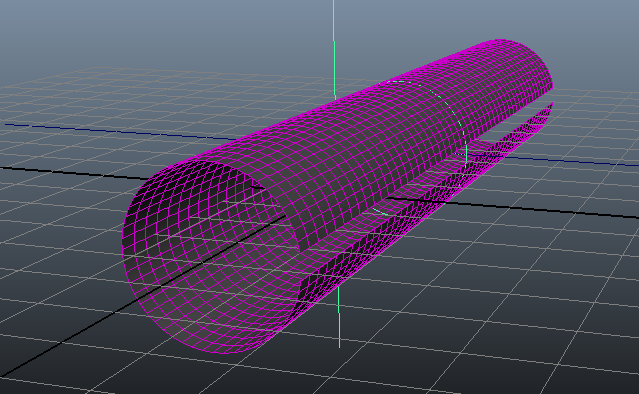
\includegraphics[width=\textwidth]{screenshots/construction01.png}
    \caption{Starting with a highly subdivided polygonal surface,
      bend it to a tube with the \emph{Deformation / Nonlinear Bend}
      tool.}
  \end{subfigure}
  \hspace{2em}
  \begin{subfigure}[t]{10cm}
    \centering
    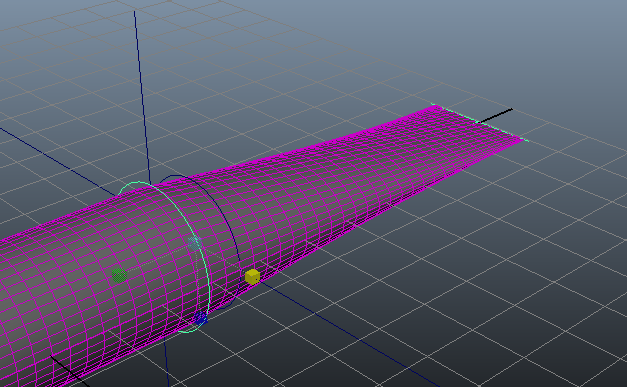
\includegraphics[width=\textwidth]{screenshots/construction02.png}
    \caption{Press down both sides of the tube using the
      \emph{Deformation / Nonlinear Flare} tool. Adjust the parameters
      of the tool so that the middle still bulges.}
  \end{subfigure}\\[2em]
  \begin{subfigure}[t]{10cm}
    \centering
    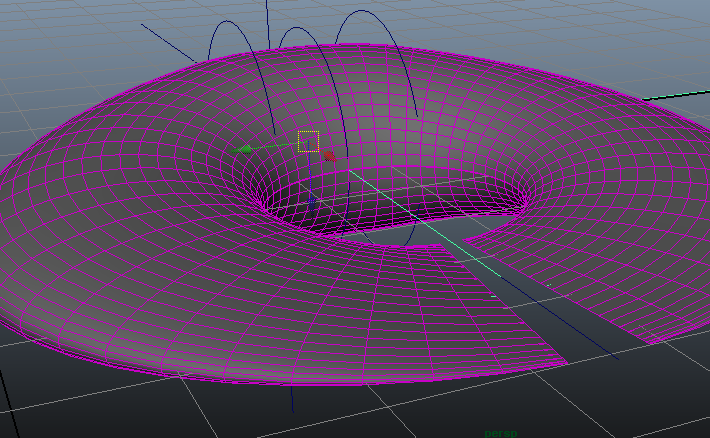
\includegraphics[width=\textwidth]{screenshots/construction03.png}
    \caption{Applying another \emph{Deformation / Nonlinear Bend}
      around the center, bring together the two “flattened” ends of
      the tube.}
  \end{subfigure}
  \hspace{2em}
  \begin{subfigure}[t]{10cm}
    \centering
    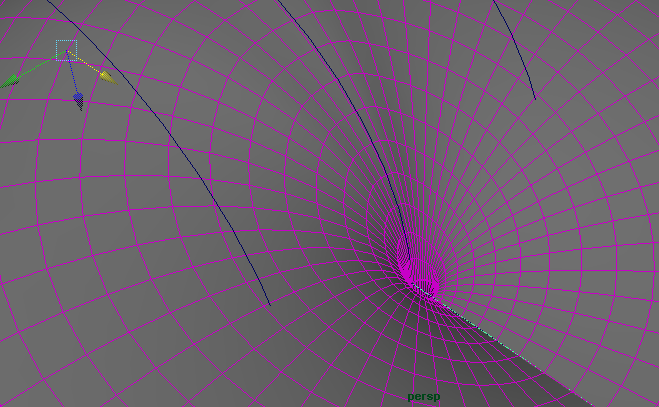
\includegraphics[width=\textwidth]{screenshots/construction04.png}
    \caption{Moving the bend handle from step (c),
      “close” the hole in the middle of the figure.}
  \end{subfigure}
\end{figure}
\end{landscape}

\subsection{Embedding the Petersen Graph}

To add the Petersen graph we projected suitable curves on the surface,
according to the construction described in
section~\ref{sec:rp2embedding}.
This is done via \emph{... > Draw on surface}.
At the self-intersection, we manually chose on which part of the surface
the curve will continue.
We subsequently thickend them, and in particular used sphere
primitives to indicate the vertices of the graph.

\begin{itemize}
  \item Which steps were used? Screenshot of this construction
\end{itemize}

\subsection{Putting Together the Animation}

In the last section we have seen how the Petersen graph can be
embedded into the $\mathbb{R}P^2$ using a planar model. In our
animation we extended the visualization to a three dimensional level
and taking advantage of being able to move around the object. Thus we
created a vehicle to give a much more intuitive feeling of the
crosscap (i.e. the $\mathbb{R}P^2$) itself and how the Peterson graph
embedding does like.

In this section we will point out the aspects our animation is showing and also briefly explain the construction process.

\subsection{Highlights of the Animation}

The first part of our animation shows the cross cap being viewed by a
camera going around the object. By seeing an object in (passive)
motion the viewer is able to get an advanced picture of the focussed
object. The route of the camera is chosen such that the viewer will
get a glance from all important perspectives and be able to make a hole
three-dimensional picture on her own.

A special highlight is that we chose the texture to indicate the
necessary selfintersection the object exhibits when immersed
in three dimensional space. This way, the viewer immediately sees that at the
intersection, the otherwise smooth gradient coloring
of the surface object suddenly breaks. At second glance she will see
how the coloring actually continues smoothly, but on the previously
obstructed “underside”.

In the second part of our animation, we show how the Petersen graph is drawn
on the surface of the cross cap. As motivation for the drawing order
we use figure \ref{fig:rp2embedding}, first drawing the lines in the
middle that can be drawn without self intersection of edges even in
the plane.

Then the camera makes a dramatic move, focussing on how each of the
remaining lines is drawn on the surface without producing any self
intersection.

%%% }}}
%%%%%%%%%%%%%%%%%%%%%%%%%%%%%%%%%%%%%%%%%%%%%%%%%%%%%%%%%%%%

%%%%%%%%%%%%%%%%%%%%%%%%%%%%%%%%%%%%%%%%%%%%%%%%%%%%%%%%%%%%
%%% Bibliographieverzeichnis {{{
\newpage
\nocite{*}
\bibliographystyle{plaindin}
\bibliography{quellen}
%%% }}}
%%%%%%%%%%%%%%%%%%%%%%%%%%%%%%%%%%%%%%%%%%%%%%%%%%%%%%%%%%%%

\end{document}

%%% vim:set fdm=marker:
